\documentclass[11pt,letterpaper]{article}
\usepackage[T1]{fontenc}
\usepackage{lmodern}
\usepackage[margin=.72in,top=.65in,bottom=.72in]{geometry}
\usepackage{amsmath,amssymb,mathtools}
\usepackage{booktabs,array,tabularx}
\usepackage{xcolor,tikz,pgfplots}
\pgfplotsset{compat=1.18,every axis/.append style={axis lines=left,grid=none,tick label style={font=\scriptsize},label style={font=\small},title style={font=\small}}}
\usepackage{microtype}
\usepackage{titlesec,fancyhdr,lastpage}
\usepackage[unicode,colorlinks=true,linkcolor=teal,urlcolor=teal]{hyperref}
\definecolor{teal}{HTML}{087E8B}
\definecolor{navy}{HTML}{152F46}
\definecolor{muted}{HTML}{526778}
\definecolor{orange}{HTML}{DB7137}
\hypersetup{pdftitle={The optic flow pathway: mathematics, logic and intuition},pdfauthor={Visual Attention Working Memory project}}
\titleformat{\section}{\sffamily\Large\bfseries\color{navy}}{\thesection.}{.5em}{}
\titleformat{\subsection}{\sffamily\normalsize\bfseries\color{teal}}{}{0pt}{}
\titlespacing*{\section}{0pt}{0pt}{12pt}
\titlespacing*{\subsection}{0pt}{9pt}{5pt}
\setlength{\parindent}{0pt}
\setlength{\parskip}{7pt}
\setlength{\headheight}{14pt}
\setlength{\emergencystretch}{2em}
\pagestyle{fancy}\fancyhf{}\renewcommand{\headrulewidth}{0pt}
\fancyfoot[L]{\sffamily\scriptsize\color{muted}VISUAL ATTENTION \& WORKING MEMORY}
\fancyfoot[R]{\sffamily\scriptsize\color{muted}\thepage\ / \pageref*{LastPage}}
\renewcommand{\footrulewidth}{.2pt}
\begin{document}
\fontsize{10.5}{13.6}\selectfont
\color{navy}
\phantomsection\addcontentsline{toc}{section}{Reading guide}\label{guide}

{\color{teal}\small\sffamily IMPLEMENTATION WALKTHROUGH\par}\medskip

{\sffamily\bfseries\fontsize{27}{32}\selectfont How our model extracts motion\par}\bigskip

\textbf{A mathematical walkthrough from pixel values to local evidence, prediction and remembered change}


The core question is simple: \textbf{which small shift makes an earlier image patch line up with a later one?} The model asks this at 100 locations, over three temporal separations. It keeps a score for every candidate shift, allowing later computations to use both the preferred motion and the alternatives.


This LaTeX document follows the actual backbone used by the 19-task suite. The source was checked against the running continuation07 source hashes on October 12, 2026. Equations reproduce that implementation; the numerical demonstrations use generated inputs on CPU. No training settings or checkpoints were changed.


\begin{center}\small\renewcommand{\arraystretch}{1.16}\setlength{\tabcolsep}{4pt}\begin{tabular}{p{0.316\linewidth}p{0.584\linewidth}}\toprule

\textbf{Operation} & \textbf{What it contributes} \\

\midrule

Pixels and overlapping crops & A local light-dark pattern at each image location. \\

Mean subtraction and windowing & Emphasis on local structure and the crop interior. \\

81 normalized shift scores & Evidence about correspondence between two observations. \\

Learned refinement and softmax & A distribution over candidate displacements. \\

Three lags and a weighted mean & Short- and longer-interval motion, plus a compact velocity estimate. \\

Prediction and temporal comparison & Whether motion continues and how local evidence changes. \\

Shared spatial attention & Which location contributes to memory and the response. \\

\bottomrule\end{tabular}\end{center}

\subsection*{How to read the equations}

Every symbol is introduced where it first appears. A scalar is one number; a vector is an ordered list; a matrix is a table of numbers. A sum adds entries, an average divides their sum by their count, and a norm measures the size of a vector. Sections 1-8 explain the motion measurement itself. Sections 9-14 explain how it becomes useful to the task. Sections 15-19 provide checked examples, theory, a glossary and sources.


{
\small\color{muted} Implementation anchors: SecondPass/\allowbreak{}StabilizedAttentionKrauzlis/\allowbreak{}model.py and SecondPass/\allowbreak{}MemoryGuidedSearch/\allowbreak{}train.py. The architecture and training-source hashes are recorded with the accompanying verification receipt.\par}


\clearpage

\section{Start with the actual input}\label{sec1}

\textbf{Intensity is a pixel value; movement is a relationship between pixel patterns at different times.}


A pixel is one addressable cell of an image. \textbf{Grayscale intensity} is its encoded light-dark value. In this input convention, 0 is black, 1 is white and 0.5 is midpoint gray. These numbers are dimensionless. A color pixel contains three component values: red, green and blue, abbreviated RGB. The motion branch takes their arithmetic mean.


\begin{equation}I_t(x,y)=\frac{X_{t,R}(x,y)+X_{t,G}(x,y)+X_{t,B}(x,y)}{3}\end{equation}

X denotes the input color image; R, G and B identify its channels. I denotes the resulting grayscale image. The subscript t selects a frame. Coordinates x and y select a column and row, with x increasing rightward and y downward. Each runs from 0 to 99. Thus I\textsubscript{5}(20,30)=0.8 means one particular pixel in frame 5 has grayscale value 0.8.


\subsection*{A numerical example}

At one pixel, RGB = (0.9, 0.6, 0.3) becomes I = 0.6. The arithmetic conversion is shared at every pixel. Equal-channel gray (0.6, 0.6, 0.6) produces the same motion input. Color information also travels through the separate appearance branch.


\begin{equation}\mathbf d=(x_2-x_1,\ y_2-y_1),\qquad \mathbf v=\mathbf d/\Delta t\end{equation}

The bold symbol d is displacement: two numbers describing a position change. If a dot moves from (20,30) to (24,28), d=(4,-2) pixels. The symbol \(\Delta\)t is the elapsed interval, and v is displacement divided by that interval. With two frame steps between the observations, v=(2,-1) pixels per frame step. A negative vertical component means upward movement.


\subsection*{Why a single image is insufficient}

A bright dot at (20,30) does not by itself tell us where it came from. A second observation supplies another pattern, and matching the patterns supplies displacement evidence. The computation operates on image arrays; its frame steps acquire physical durations only when a presentation rate is specified.


{
\small\color{muted} Source: model.py, forward(), lines 88-96. This document uses t as an integer frame index throughout.\par}


\clearpage

\section{Where the model looks}\label{sec2}

\textbf{A site is one position on the 10 by 10 analysis grid.}


There are 100 sites: 10 rows and 10 columns. Each site has a 24 by 24 grayscale crop containing 576 values. Crops start 10 pixels apart, so nearby sites see some of the same pixels. That shared input is what \textbf{overlapping evidence} means.


\begin{equation}x=10c-7+a,\qquad y=10r-7+b,\qquad i=10r+c\end{equation}

Here r and c are site row and column, each 0 through 9. The single index i labels the site, 0 through 99. Crop coordinates a and b each run from 0 through 23. The crop center is (10c+4.5, 10r+4.5). For site (4,4), the crop covers x=33 through 56 and y=33 through 56. Its neighboring crop at (4,5) covers x=43 through 66.


\begin{center}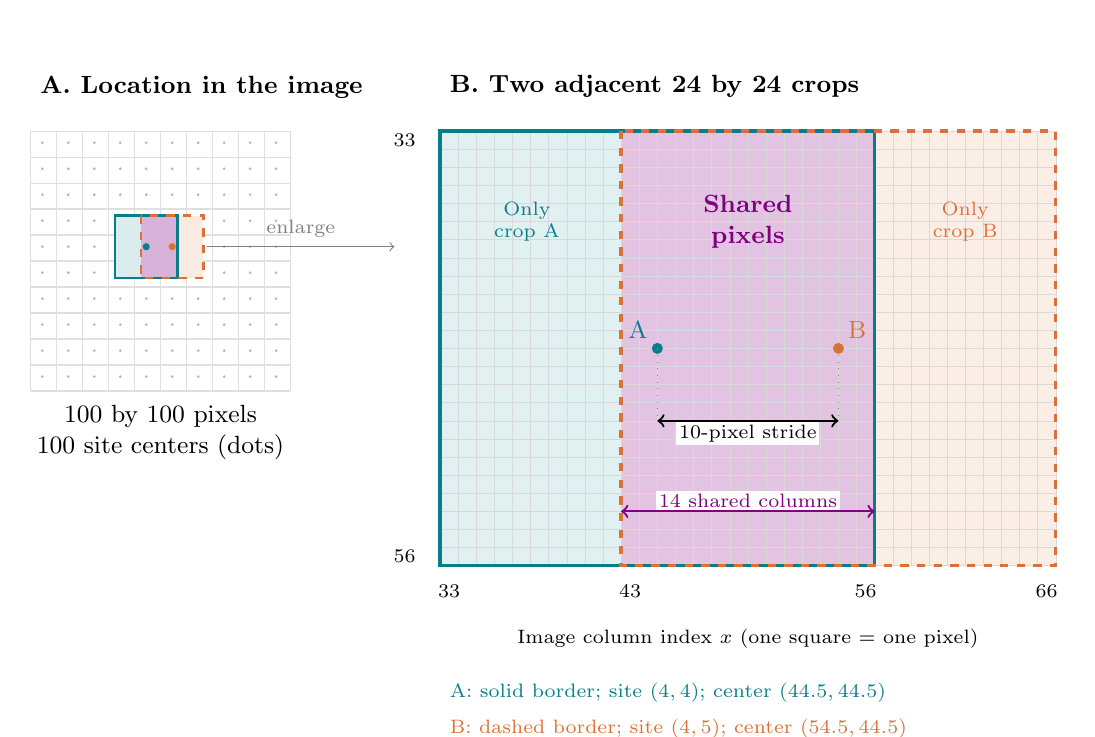
\begin{tikzpicture}[font=\small]
\begin{scope}[x=.033cm,y=-.033cm]
\node[anchor=west,font=\small\bfseries] at (0,-17){A. Location in the image};
\foreach \v in {0,10,...,100}{\draw[gray!25] (\v,0)--(\v,100);\draw[gray!25] (0,\v)--(100,\v);}
\foreach \r in {0,...,9}{\foreach \c in {0,...,9}{\fill[gray!55] (10*\c+4.5,10*\r+4.5) circle (.55pt);}}
\fill[teal!15] (32.5,32.5) rectangle (56.5,56.5);
\fill[orange!15] (42.5,32.5) rectangle (66.5,56.5);
\fill[violet!30] (42.5,32.5) rectangle (56.5,56.5);
\draw[teal,thick] (32.5,32.5) rectangle (56.5,56.5);
\draw[orange,thick,dashed] (42.5,32.5) rectangle (66.5,56.5);
\fill[teal] (44.5,44.5) circle (1.3pt);\fill[orange] (54.5,44.5) circle (1.3pt);
\node[align=center] at (50,116){100 by 100 pixels\\100 site centers (dots)};
\draw[->,gray] (68,44.5)--(140,44.5) node[midway,above,font=\scriptsize]{enlarge};
\end{scope}
\begin{scope}[xshift=5.2cm,x=.23cm,y=-.23cm]
\node[anchor=west,font=\small\bfseries] at (0,-2.45){B. Two adjacent 24 by 24 crops};
\fill[teal!12] (0,0) rectangle (10,24);
\fill[violet!23] (10,0) rectangle (24,24);
\fill[orange!12] (24,0) rectangle (34,24);
\foreach \v in {0,...,34}{\draw[gray!30,very thin] (\v,0)--(\v,24);}
\foreach \v in {0,...,24}{\draw[gray!30,very thin] (0,\v)--(34,\v);}
\draw[teal,line width=1.2pt] (0,0) rectangle (24,24);
\draw[orange,line width=1.2pt,dashed] (10,0) rectangle (34,24);
\node[align=center,font=\scriptsize,text=teal] at (4.8,5){Only\\crop A};
\node[align=center,font=\small\bfseries,text=violet] at (17,5){Shared\\pixels};
\node[align=center,font=\scriptsize,text=orange] at (29,5){Only\\crop B};
\fill[teal] (12,12) circle (2pt);\node[above left,text=teal] at (12,12){A};
\fill[orange] (22,12) circle (2pt);\node[above right,text=orange] at (22,12){B};
\draw[gray,dotted] (12,12)--(12,16);\draw[gray,dotted] (22,12)--(22,16);
\draw[<->,thick] (12,16)--(22,16) node[midway,below,fill=white,inner sep=1pt,font=\scriptsize]{10-pixel stride};
\draw[<->,violet,thick] (10,21)--(24,21) node[midway,above,fill=white,inner sep=1pt,font=\scriptsize]{14 shared columns};
\node[anchor=east,font=\scriptsize] at (-.8,.5){33};
\node[anchor=east,font=\scriptsize] at (-.8,23.5){56};
\foreach \x/\lab in {.5/33,10.5/43,23.5/56,33.5/66}{\node[below,font=\scriptsize] at (\x,24.5){\lab};}
\node[font=\scriptsize] at (17,28){Image column index $x$ (one square = one pixel)};
\node[anchor=west,text=teal,font=\scriptsize] at (0,31){A: solid border; site $(4,4)$; center $(44.5,44.5)$};
\node[anchor=west,text=orange,font=\scriptsize] at (0,33){B: dashed border; site $(4,5)$; center $(54.5,44.5)$};
\end{scope}\end{tikzpicture}\end{center}

{
\small\color{muted} Figure 1. Left: where two neighboring sites lie in the full image. Right: the same crops enlarged to show individual pixels. Crop A covers columns 33-56; crop B covers 43-66. Both cover rows 33-56. Their shared region contains 14 columns by 24 rows = 336 pixels. Their centers are 10 pixels apart.\par}


The model first subtracts 0.5 from the full grayscale image, then pads it with seven zeros on every side. A padded value therefore represents midpoint gray in the original input convention. Padding lets the same crop rule work at the outermost sites.


\textbf{Why this scale?} A larger local neighborhood lets moving structure remain available to matching. A smaller stride makes neighboring measurements overlap. The values 24 and 10 are fixed architectural choices: training adjusts learned weights, but it does not resize these crops or relocate the grid. The attention display assigns each site a 10 by 10 image tile; its motion measurement uses the larger crop.


\clearpage

\section{Prepare the crop}\label{sec3}

\textbf{Remove the local average and gradually reduce the influence of the boundary.}


Let Q\textsubscript{t,i}(a,b) be the crop after the global subtraction of 0.5 and padding. Compute its mean over all 576 entries. Subtracting that mean turns brighter-than-average entries positive and darker-than-average entries negative.


\begin{equation}\overline Q_{t,i}=\frac{1}{576}\sum_{a=0}^{23}\sum_{b=0}^{23}Q_{t,i}(a,b)\end{equation}

\begin{equation}P_{t,i}(a,b)=[Q_{t,i}(a,b)-\overline Q_{t,i}]\,w(a)w(b)\end{equation}

\begin{equation}w(n)=\frac12\left[1-\cos\left(\frac{2\pi n}{23}\right)\right],\quad n=0,\ldots,23\end{equation}

P names the prepared crop. The function w is a nonperiodic Hann window: it is zero at the endpoints and close to one near the center. Multiplying a horizontal weight by a vertical weight gives the two-dimensional weight at each crop pixel. The symbol \(\pi\) is the circle constant; cosine gives the smooth taper.


\begin{center}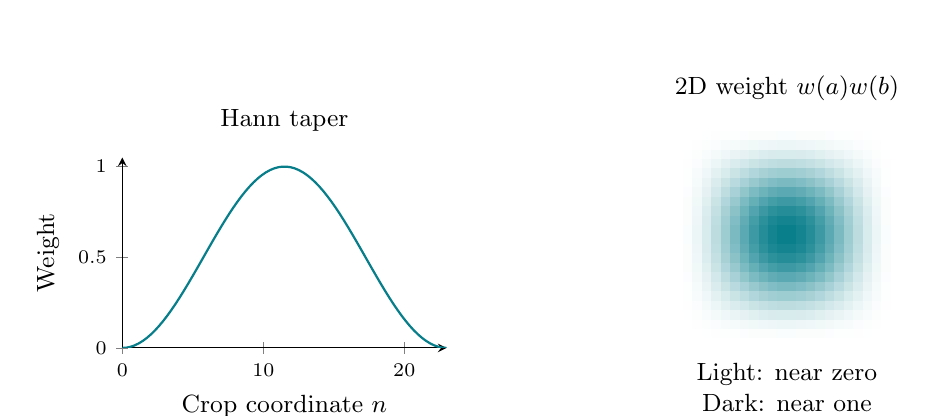
\begin{tikzpicture}
\begin{axis}[width=.47\linewidth,height=4.0cm,xmin=0,xmax=23,ymin=0,ymax=1.05,xlabel={Crop coordinate $n$},ylabel={Weight},title={Hann taper}]
\addplot[teal,thick,domain=0:23,samples=80]{.5*(1-cos(deg(2*pi*x/23)))};
\end{axis}
\begin{scope}[xshift=7.0cm]
\foreach \a in {0,...,23}{\foreach \b in {0,...,23}{\pgfmathsetmacro{\shade}{100*.5*(1-cos(360*\a/23))*.5*(1-cos(360*\b/23))}\fill[teal!\shade!white] (\a*.12,\b*.12) rectangle ++(.12,.12);}}
\node[font=\small] at (1.44,3.3){2D weight $w(a)w(b)$};
\node[font=\small,align=center] at (1.44,-.5){Light: near zero\\Dark: near one};
\end{scope}\end{tikzpicture}\end{center}

{
\small\color{muted} Figure 2. Native vector plots of the one-dimensional Hann taper and its two-dimensional product. Windowing emphasizes the crop interior.\par}


\textbf{Why subtract the mean?} A uniform brightness level would contribute a broad positive match at many shifts. Centering emphasizes variation within the crop. Adding the same constant everywhere in an interior crop leaves the prepared pattern unchanged. At image borders, padding also participates in the mean.


\textbf{Why taper?} A sharply cut edge of a crop can act like an artificial image edge. Windowing emphasizes central structure and makes boundary values fade. Both observations receive a window fixed to the crop coordinates. A moving feature therefore receives slightly different weights as it moves; even a correct match can score below one.


{
\small\color{muted} Subtraction and tapering are distinct operations. The crop has zero mean immediately after subtraction; multiplication by the nonuniform window can change that mean again.\par}


\clearpage

\section{Ask 81 correspondence questions}\label{sec4}

\textbf{For each candidate displacement, multiply aligned values and add the products.}


Choose one site and two prepared crops. Call the earlier crop A and the current crop B. A candidate displacement d=(d\textsubscript{x},d\textsubscript{y}) says that structure at (a,b) in A should appear at (a+d\textsubscript{x},b+d\textsubscript{y}) in B.


\textbf{Where do -4 and +4 come from?} The implementation chooses a search radius R=4 pixels along each axis. R is a fixed hyperparameter: a setting selected when building the model. It specifies which possible shifts the model measures. The code explicitly constructs the integers -4, -3, -2, -1, 0, 1, 2, 3, 4. Minus means left/\allowbreak{}up, plus means right/\allowbreak{}down, and zero means no shift along that axis. There are nine choices because both endpoints and zero are included.


\begin{equation}\#\mathrm{offsets\ per\ axis}=2R+1,\qquad K=(2R+1)^2=81\quad\mathrm{when}\ R=4\end{equation}

K is the number of horizontal/\allowbreak{}vertical combinations. Thus \textbf{4 is chosen; 9 and 81 are derived}. A radius of 2 would give 25 pairs; a radius of 8 would give 289. A wider range represents larger displacements but expands the retained score population and downstream feature vectors. Radius 4 limits each component of the estimated displacement to [-4,4] for every lag. It is independent of the 24-pixel crop size; it is not derived from that crop size or a neuroscience equation. No radius-selection comparison is documented in the inspected model notes.


\begin{equation}N(\mathbf d)=\sum_{a,b} A(a,b)\,B(a+d_x,b+d_y)\end{equation}

N is the unnormalized correlation score. The summation adds products over crop coordinates. For this equation, treat values beyond the 24 by 24 crop as zero. A positive value meeting a positive value contributes positively; two negative values also contribute positively. Opposite signs reduce the score. A displacement that aligns the light-dark structure tends to produce a large sum.


\subsection*{Work through a tiny one-dimensional example}

Take an already prepared row A=[0,1,-1,0,0] and a later row B=[0,0,1,-1,0]. At displacement 0, the nonzero product is (-1) times 1, giving N(0)=-1. At displacement +1, the aligned products are 1 times 1 and (-1) times (-1), giving N(+1)=2. The larger score supports a one-pixel shift to the right. The two-dimensional operation performs the same arithmetic in both axes.


\begin{equation}\mathcal D=\{(d_x,d_y):d_x,d_y\in\{-4,-3,\ldots,4\}\}\end{equation}

The symbol D in this equation is the set of candidate shifts. Arranging the scores as a 9 by 9 table gives a \textbf{displacement map}. Its rows indicate vertical shifts and its columns horizontal shifts. It is a map of motion alternatives for one image location. Repeating the calculation at all 100 sites gives 100 such tables for each time lag.


\textbf{Why keep all scores?} A repeating pattern may align at several shifts. A long straight edge can constrain motion across the edge while leaving motion along it ambiguous. Keeping the whole table preserves these alternatives for later computation. Correlation volumes also appear in learned optical-flow systems such as FlowNet [1]. Our score volume is built directly from prepared grayscale crops.


\clearpage

\section{Separate shape from signal strength}\label{sec5}

\textbf{Normalization measures alignment; a separate factor records how much prepared signal is present.}


\begin{equation}E_A=\sum_{a,b}A(a,b)^2,\quad E_B=\sum_{a,b}B(a,b)^2,\quad z=\sqrt{E_AE_B}\end{equation}

\begin{equation}C(\mathbf d)=\frac{N(\mathbf d)}{\max(z,10^{-8})},\qquad r=\frac{z}{z+0.01}\end{equation}

E\textsubscript{A} and E\textsubscript{B} are sums of squared prepared pixel values, called crop energies. Squaring makes both positive and negative deviations contribute. z is the geometric mean of the two energies. C is the normalized correspondence score. The maximum in its denominator prevents division by a value smaller than 10\textsuperscript{-8}. The scalar r, between zero and one, is the code's energy-based reliability factor.


In the small row example, both energies equal 2, so z=2. The correct-shift score becomes 2/\allowbreak{}2=1 and the zero-shift score becomes -1/\allowbreak{}2=-0.5. If A is multiplied by a positive factor a and B by a positive factor b, the product sum and z both scale by ab. Their ratio stays the same when the numerical floor is inactive.


\begin{center}\small\renewcommand{\arraystretch}{1.16}\setlength{\tabcolsep}{4pt}\begin{tabular}{p{0.110\linewidth}p{0.312\linewidth}p{0.478\linewidth}}\toprule

\textbf{z} & \textbf{r = z /\allowbreak{} (z + 0.01)} & \textbf{Interpretation} \\

\midrule

0 & 0 & No prepared variation in at least one crop. \\

0.01 & 0.5 & The energy factor gives half weight. \\

0.09 & 0.9 & Substantial prepared signal. \\

0.99 & 0.99 & The factor is close to its upper limit. \\

\bottomrule\end{tabular}\end{center}

\textbf{What exactly is normalized?} The denominator uses the energies of the two full prepared crops and is shared across all candidate shifts. The code does not recompute a different denominator or a different local mean for each overlap region. This precise rule matters when reproducing the score.


\textbf{What does reliability mean here?} It measures available prepared-image energy. Rich random noise can have high energy, and a periodic texture can have high energy but several plausible shifts. The displacement table carries match structure; r supplies a separate signal-strength measure. At flat midpoint gray, both C and r are exactly zero.


{
\small\color{muted} Code names: costs = C; valid = r. These are similarity scores, so larger means a better match. The name valid denotes energy weighting, not an explicit check that a full temporal lag has elapsed.\par}


\clearpage

\section{The FFT computes the same sums}\label{sec6}

\textbf{The Fourier transform changes the arithmetic, while the question remains alignment under a shift.}


A Fourier transform expresses an array through sinusoidal components. Each component has a magnitude and a phase; phase specifies its alignment. For a finite array the transform is an invertible change of coordinates. FFT means fast Fourier transform, an efficient algorithm for calculating this change. Multiplication of Fourier coefficients can compute all the correlation shifts together.


\begin{equation}\widehat A=\mathcal F_{32}(A),\qquad \widehat B=\mathcal F_{32}(B)\end{equation}

\begin{equation}N_{32}=\mathcal F_{32}^{-1}(\overline{\widehat A}\,\widehat B)\end{equation}

The calligraphic F denotes the two-dimensional Fourier transform on a 32 by 32 array. A hat denotes its coefficients. The overbar here means complex conjugation: reverse the sign of the imaginary component. It has a different role from the crop-mean bar on section 3, because its operand is a complex coefficient. The inverse transform returns a real 32 by 32 table of shift scores [2].


\subsection*{Why the order matters}

Conjugating the \textbf{earlier} spectrum and multiplying by the later spectrum produces the forward-shift convention on section 4. A rightward displacement peaks at positive d\textsubscript{x}. Swapping which spectrum is conjugated reverses that convention. In the code, spectra[:,ix].conj() is the earlier term and spectra is the current term.


\begin{equation}\operatorname{index}(d_x,d_y)=32(d_y\bmod32)+(d_x\bmod32)\end{equation}

The operator mod gives a remainder between 0 and 31. It maps a negative shift such as -1 to array index 31. Flattening the 32 by 32 result then uses row times 32 plus column. The model retrieves only the 81 entries for shifts -4 through +4.


\subsection*{Why pad 24 to 32?}

A discrete FFT gives circular correlation: indices wrap at 32. Each crop occupies coordinates 0 through 23 and the remaining eight positions contain zeros. For the retained shifts of at most four pixels per axis, wrapped signal cannot meet the opposite edge of the other 24-pixel crop. Consequently these retained entries equal the finite, zero-extended product sums. Full correlation at every possible shift would require a larger array.


{
\small\color{muted} Independent CPU check: all 81 retained normalized FFT scores matched explicit sums; maximum absolute difference 4.5e-08. The checked code uses rfft2/\allowbreak{}irfft2 to exploit the symmetry of real-valued inputs.\par}


\clearpage

\section{Turn scores into a population}\label{sec7}

\textbf{A small learned correction adjusts the score map; softmax makes the weights sum to one.}


\begin{equation}\widetilde C=C+0.1\,f_\theta(C),\qquad f_\theta:\ 1\to4\to1\ \mathrm{channels}\end{equation}

C is one 9 by 9 score map. The learned function f\textsubscript{\(\theta\)} applies a 3 by 3 convolution from one channel to four, a GELU nonlinearity, and another 3 by 3 convolution back to one. A convolution forms local weighted sums shared across map positions. Here those positions are \textbf{candidate displacements}. A neighboring cell represents a similar possible shift. GELU makes the correction depend nonlinearly on those sums.


The same correction network is used at every image site, time and lag. Both layers use padding one to preserve 9 by 9 shape. The last layer starts with zero weights and bias, so the initial correction is exactly zero. The fixed factor 0.1 scales its contribution. The learned parameters \(\theta\) can reshape nearby peaks as task learning proceeds.


\begin{equation}p_k=\frac{\exp(\widetilde C_k/\tau_\ell)}{\sum_{j=1}^{81}\exp(\widetilde C_j/\tau_\ell)},\qquad \sum_{k=1}^{81}p_k=1\end{equation}

k indexes one candidate shift; j indexes all candidates in the denominator. p\textsubscript{k} is its normalized weight. The positive number \(\tau\)\textsubscript{\(\ell\)}, called temperature, is separate for each lag \(\ell\). It starts at 0.04 and is computed as exp of a learned parameter, clamped to [0.015, 0.2]. A smaller temperature magnifies score differences before normalization.


\begin{center}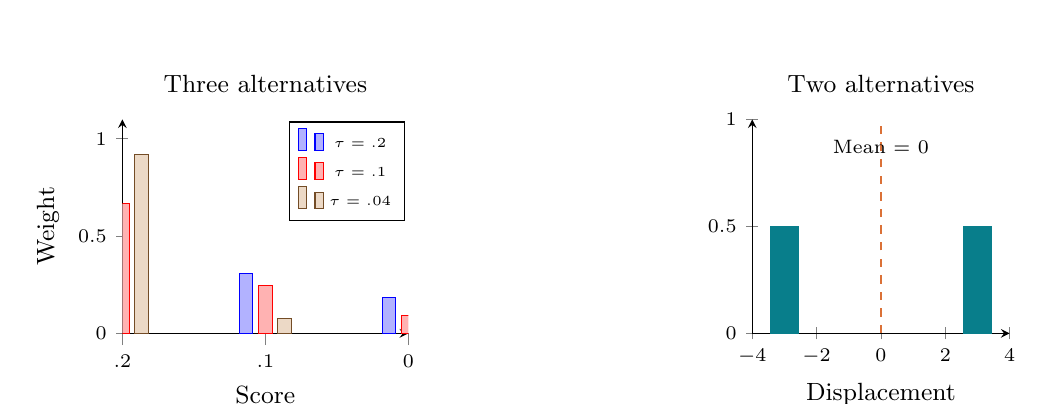
\begin{tikzpicture}
\begin{axis}[width=.43\linewidth,height=4.3cm,ybar,bar width=5pt,ymin=0,ymax=1.1,xtick={0,1,2},xticklabels={$.2$,$.1$,$0$},xlabel={Score},ylabel={Weight},title={Three alternatives},legend style={font=\tiny,at={(.99,.99)},anchor=north east}]
\addplot coordinates{(0,.50648)(1,.3072)(2,.18632)};\addlegendentry{$\tau=.2$}
\addplot coordinates{(0,.66524)(1,.24473)(2,.09003)};\addlegendentry{$\tau=.1$}
\addplot coordinates{(0,.91842)(1,.07539)(2,.00619)};\addlegendentry{$\tau=.04$}
\end{axis}
\begin{axis}[at={(8.0cm,0)},width=.40\linewidth,height=4.3cm,ymin=0,ymax=1,xmin=-4,xmax=4,xlabel={Displacement},title={Two alternatives},ytick={0,.5,1}]
\addplot[ybar,bar width=10pt,fill=teal,draw=teal]coordinates{(-3,.5)(3,.5)};
\addplot[orange,dashed]coordinates{(0,0)(0,1)};
\node[font=\scriptsize,anchor=north] at (axis cs:0,.95){Mean = 0};
\end{axis}\end{tikzpicture}\end{center}

{
\small\color{muted} Figure 3. Left: a three-alternative teaching example. Right: a distribution can express two opposing shifts even when its mean is zero.\par}


The odds ratio is exp[(\(\widetilde C\)\textsubscript{i}-\(\widetilde C\)\textsubscript{j})/\allowbreak{}\(\tau\)]. A score advantage of 0.1 at \(\tau\)=0.04 gives about 12.2 times as much weight. The term \textbf{population} means the entire 81-number vector, with each coordinate assigned a candidate displacement. These normalized weights can be used as a discrete distribution in subsequent arithmetic.


\clearpage

\section{Three lags, one velocity convention}\label{sec8}

\textbf{Displacement accumulated over four frames must be divided by four to obtain pixels per frame.}


\begin{equation}s(t,\ell)=\max(t-\ell,0),\qquad \ell\in\{1,2,4\}\end{equation}

s is the earlier frame index. The model compares current frame t to frames one, two and four steps earlier. When the requested earlier index would be negative, it uses frame zero. Each lag has its own 81-entry population p\textsubscript{t,\(\ell\),i}. The index i identifies the spatial site.


\begin{equation}\widehat{\mathbf d}_{t,\ell,i}=\sum_{k=1}^{81}p_{t,\ell,i,k}\,\mathbf d_k,\qquad \widehat{\mathbf v}_{t,\ell,i}=\widehat{\mathbf d}_{t,\ell,i}/\ell\end{equation}

The hat marks an estimate. d\textsubscript{k} is the fixed two-component displacement for candidate k. Multiply each candidate vector by its weight and add: this is the expected displacement. Dividing by the nominal lag gives velocity. For steady rightward motion of one pixel per frame, the expected displacement peaks are (1,0), (2,0) and (4,0). All three imply velocity (1,0).


\begin{center}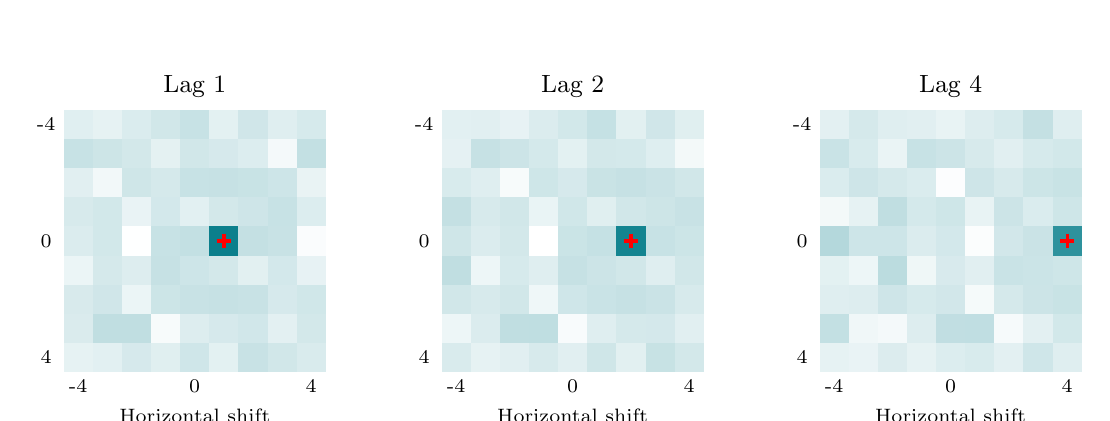
\begin{tikzpicture}[x=.37cm,y=-.37cm]
\begin{scope}[xshift=0.0cm]
\node[font=\small] at (4,-1.3){Lag 1};
\fill[teal!12.426!white] (-0.5,-0.5) rectangle (0.5,0.5);
\fill[teal!10.291!white] (0.5,-0.5) rectangle (1.5,0.5);
\fill[teal!15.016!white] (1.5,-0.5) rectangle (2.5,0.5);
\fill[teal!18.800!white] (2.5,-0.5) rectangle (3.5,0.5);
\fill[teal!22.562!white] (3.5,-0.5) rectangle (4.5,0.5);
\fill[teal!11.207!white] (4.5,-0.5) rectangle (5.5,0.5);
\fill[teal!19.182!white] (5.5,-0.5) rectangle (6.5,0.5);
\fill[teal!12.996!white] (6.5,-0.5) rectangle (7.5,0.5);
\fill[teal!16.659!white] (7.5,-0.5) rectangle (8.5,0.5);
\fill[teal!22.672!white] (-0.5,0.5) rectangle (0.5,1.5);
\fill[teal!20.332!white] (0.5,0.5) rectangle (1.5,1.5);
\fill[teal!17.830!white] (1.5,0.5) rectangle (2.5,1.5);
\fill[teal!10.834!white] (2.5,0.5) rectangle (3.5,1.5);
\fill[teal!18.689!white] (3.5,0.5) rectangle (4.5,1.5);
\fill[teal!16.738!white] (4.5,0.5) rectangle (5.5,1.5);
\fill[teal!14.059!white] (5.5,0.5) rectangle (6.5,1.5);
\fill[teal!4.307!white] (6.5,0.5) rectangle (7.5,1.5);
\fill[teal!24.374!white] (7.5,0.5) rectangle (8.5,1.5);
\fill[teal!12.210!white] (-0.5,1.5) rectangle (0.5,2.5);
\fill[teal!5.067!white] (0.5,1.5) rectangle (1.5,2.5);
\fill[teal!19.470!white] (1.5,1.5) rectangle (2.5,2.5);
\fill[teal!17.042!white] (2.5,1.5) rectangle (3.5,2.5);
\fill[teal!22.651!white] (3.5,1.5) rectangle (4.5,2.5);
\fill[teal!23.262!white] (4.5,1.5) rectangle (5.5,2.5);
\fill[teal!22.089!white] (5.5,1.5) rectangle (6.5,2.5);
\fill[teal!20.088!white] (6.5,1.5) rectangle (7.5,2.5);
\fill[teal!9.079!white] (7.5,1.5) rectangle (8.5,2.5);
\fill[teal!16.031!white] (-0.5,2.5) rectangle (0.5,3.5);
\fill[teal!18.023!white] (0.5,2.5) rectangle (1.5,3.5);
\fill[teal!8.935!white] (1.5,2.5) rectangle (2.5,3.5);
\fill[teal!17.637!white] (2.5,2.5) rectangle (3.5,3.5);
\fill[teal!11.557!white] (3.5,2.5) rectangle (4.5,3.5);
\fill[teal!17.929!white] (4.5,2.5) rectangle (5.5,3.5);
\fill[teal!19.934!white] (5.5,2.5) rectangle (6.5,3.5);
\fill[teal!22.788!white] (6.5,2.5) rectangle (7.5,3.5);
\fill[teal!14.000!white] (7.5,2.5) rectangle (8.5,3.5);
\fill[teal!14.387!white] (-0.5,3.5) rectangle (0.5,4.5);
\fill[teal!18.083!white] (0.5,3.5) rectangle (1.5,4.5);
\fill[teal!0.339!white] (1.5,3.5) rectangle (2.5,4.5);
\fill[teal!22.748!white] (2.5,3.5) rectangle (3.5,4.5);
\fill[teal!24.332!white] (3.5,3.5) rectangle (4.5,4.5);
\fill[teal!98.859!white] (4.5,3.5) rectangle (5.5,4.5);
\fill[teal!23.932!white] (5.5,3.5) rectangle (6.5,4.5);
\fill[teal!22.200!white] (6.5,3.5) rectangle (7.5,4.5);
\fill[teal!2.130!white] (7.5,3.5) rectangle (8.5,4.5);
\fill[teal!8.029!white] (-0.5,4.5) rectangle (0.5,5.5);
\fill[teal!16.878!white] (0.5,4.5) rectangle (1.5,5.5);
\fill[teal!13.635!white] (1.5,4.5) rectangle (2.5,5.5);
\fill[teal!23.250!white] (2.5,4.5) rectangle (3.5,5.5);
\fill[teal!20.070!white] (3.5,4.5) rectangle (4.5,5.5);
\fill[teal!17.929!white] (4.5,4.5) rectangle (5.5,5.5);
\fill[teal!11.741!white] (5.5,4.5) rectangle (6.5,5.5);
\fill[teal!17.627!white] (6.5,4.5) rectangle (7.5,5.5);
\fill[teal!9.778!white] (7.5,4.5) rectangle (8.5,5.5);
\fill[teal!15.968!white] (-0.5,5.5) rectangle (0.5,6.5);
\fill[teal!19.025!white] (0.5,5.5) rectangle (1.5,6.5);
\fill[teal!8.016!white] (1.5,5.5) rectangle (2.5,6.5);
\fill[teal!20.451!white] (2.5,5.5) rectangle (3.5,6.5);
\fill[teal!22.287!white] (3.5,5.5) rectangle (4.5,6.5);
\fill[teal!23.263!white] (4.5,5.5) rectangle (5.5,6.5);
\fill[teal!22.386!white] (5.5,5.5) rectangle (6.5,6.5);
\fill[teal!16.714!white] (6.5,5.5) rectangle (7.5,6.5);
\fill[teal!18.895!white] (7.5,5.5) rectangle (8.5,6.5);
\fill[teal!15.148!white] (-0.5,6.5) rectangle (0.5,7.5);
\fill[teal!25.516!white] (0.5,6.5) rectangle (1.5,7.5);
\fill[teal!25.559!white] (1.5,6.5) rectangle (2.5,7.5);
\fill[teal!3.194!white] (2.5,6.5) rectangle (3.5,7.5);
\fill[teal!13.947!white] (3.5,6.5) rectangle (4.5,7.5);
\fill[teal!16.740!white] (4.5,6.5) rectangle (5.5,7.5);
\fill[teal!18.519!white] (5.5,6.5) rectangle (6.5,7.5);
\fill[teal!11.403!white] (6.5,6.5) rectangle (7.5,7.5);
\fill[teal!17.773!white] (7.5,6.5) rectangle (8.5,7.5);
\fill[teal!10.290!white] (-0.5,7.5) rectangle (0.5,8.5);
\fill[teal!11.575!white] (0.5,7.5) rectangle (1.5,8.5);
\fill[teal!16.755!white] (1.5,7.5) rectangle (2.5,8.5);
\fill[teal!12.736!white] (2.5,7.5) rectangle (3.5,8.5);
\fill[teal!19.304!white] (3.5,7.5) rectangle (4.5,8.5);
\fill[teal!11.209!white] (4.5,7.5) rectangle (5.5,8.5);
\fill[teal!22.343!white] (5.5,7.5) rectangle (6.5,8.5);
\fill[teal!18.603!white] (6.5,7.5) rectangle (7.5,8.5);
\fill[teal!15.248!white] (7.5,7.5) rectangle (8.5,8.5);
\draw[red,very thick] (4.75,4)--(5.25,4);\draw[red,very thick] (5,3.75)--(5,4.25);
\node[font=\scriptsize] at (0,9){-4};\node[font=\scriptsize] at (-1.1,0){-4};
\node[font=\scriptsize] at (4,9){0};\node[font=\scriptsize] at (-1.1,4){0};
\node[font=\scriptsize] at (8,9){4};\node[font=\scriptsize] at (-1.1,8){4};
\node[font=\scriptsize] at (4,10){Horizontal shift};\end{scope}
\begin{scope}[xshift=4.8cm]
\node[font=\small] at (4,-1.3){Lag 2};
\fill[teal!11.624!white] (-0.5,-0.5) rectangle (0.5,0.5);
\fill[teal!12.316!white] (0.5,-0.5) rectangle (1.5,0.5);
\fill[teal!9.770!white] (1.5,-0.5) rectangle (2.5,0.5);
\fill[teal!14.583!white] (2.5,-0.5) rectangle (3.5,0.5);
\fill[teal!18.052!white] (3.5,-0.5) rectangle (4.5,0.5);
\fill[teal!23.394!white] (4.5,-0.5) rectangle (5.5,0.5);
\fill[teal!11.669!white] (5.5,-0.5) rectangle (6.5,0.5);
\fill[teal!19.195!white] (6.5,-0.5) rectangle (7.5,0.5);
\fill[teal!12.615!white] (7.5,-0.5) rectangle (8.5,0.5);
\fill[teal!10.605!white] (-0.5,0.5) rectangle (0.5,1.5);
\fill[teal!22.958!white] (0.5,0.5) rectangle (1.5,1.5);
\fill[teal!20.617!white] (1.5,0.5) rectangle (2.5,1.5);
\fill[teal!17.436!white] (2.5,0.5) rectangle (3.5,1.5);
\fill[teal!11.201!white] (3.5,0.5) rectangle (4.5,1.5);
\fill[teal!17.842!white] (4.5,0.5) rectangle (5.5,1.5);
\fill[teal!17.205!white] (5.5,0.5) rectangle (6.5,1.5);
\fill[teal!13.197!white] (6.5,0.5) rectangle (7.5,1.5);
\fill[teal!5.029!white] (7.5,0.5) rectangle (8.5,1.5);
\fill[teal!15.703!white] (-0.5,1.5) rectangle (0.5,2.5);
\fill[teal!12.873!white] (0.5,1.5) rectangle (1.5,2.5);
\fill[teal!3.359!white] (1.5,1.5) rectangle (2.5,2.5);
\fill[teal!19.676!white] (2.5,1.5) rectangle (3.5,2.5);
\fill[teal!16.694!white] (3.5,1.5) rectangle (4.5,2.5);
\fill[teal!22.040!white] (4.5,1.5) rectangle (5.5,2.5);
\fill[teal!22.977!white] (5.5,1.5) rectangle (6.5,2.5);
\fill[teal!21.619!white] (6.5,1.5) rectangle (7.5,2.5);
\fill[teal!18.786!white] (7.5,1.5) rectangle (8.5,2.5);
\fill[teal!23.999!white] (-0.5,2.5) rectangle (0.5,3.5);
\fill[teal!16.371!white] (0.5,2.5) rectangle (1.5,3.5);
\fill[teal!18.697!white] (1.5,2.5) rectangle (2.5,3.5);
\fill[teal!8.790!white] (2.5,2.5) rectangle (3.5,3.5);
\fill[teal!18.861!white] (3.5,2.5) rectangle (4.5,3.5);
\fill[teal!12.681!white] (4.5,2.5) rectangle (5.5,3.5);
\fill[teal!18.786!white] (5.5,2.5) rectangle (6.5,3.5);
\fill[teal!20.307!white] (6.5,2.5) rectangle (7.5,3.5);
\fill[teal!22.129!white] (7.5,2.5) rectangle (8.5,3.5);
\fill[teal!19.617!white] (-0.5,3.5) rectangle (0.5,4.5);
\fill[teal!14.399!white] (0.5,3.5) rectangle (1.5,4.5);
\fill[teal!17.972!white] (1.5,3.5) rectangle (2.5,4.5);
\fill[teal!0.152!white] (2.5,3.5) rectangle (3.5,4.5);
\fill[teal!21.317!white] (3.5,3.5) rectangle (4.5,4.5);
\fill[teal!23.448!white] (4.5,3.5) rectangle (5.5,4.5);
\fill[teal!95.611!white] (5.5,3.5) rectangle (6.5,4.5);
\fill[teal!22.705!white] (6.5,3.5) rectangle (7.5,4.5);
\fill[teal!20.488!white] (7.5,3.5) rectangle (8.5,4.5);
\fill[teal!25.603!white] (-0.5,4.5) rectangle (0.5,5.5);
\fill[teal!7.221!white] (0.5,4.5) rectangle (1.5,5.5);
\fill[teal!16.594!white] (1.5,4.5) rectangle (2.5,5.5);
\fill[teal!13.096!white] (2.5,4.5) rectangle (3.5,5.5);
\fill[teal!23.055!white] (3.5,4.5) rectangle (4.5,5.5);
\fill[teal!20.595!white] (4.5,4.5) rectangle (5.5,5.5);
\fill[teal!18.777!white] (5.5,4.5) rectangle (6.5,5.5);
\fill[teal!12.949!white] (6.5,4.5) rectangle (7.5,5.5);
\fill[teal!18.627!white] (7.5,4.5) rectangle (8.5,5.5);
\fill[teal!18.570!white] (-0.5,5.5) rectangle (0.5,6.5);
\fill[teal!16.002!white] (0.5,5.5) rectangle (1.5,6.5);
\fill[teal!18.698!white] (1.5,5.5) rectangle (2.5,6.5);
\fill[teal!6.387!white] (2.5,5.5) rectangle (3.5,6.5);
\fill[teal!19.349!white] (3.5,5.5) rectangle (4.5,6.5);
\fill[teal!21.953!white] (4.5,5.5) rectangle (5.5,6.5);
\fill[teal!22.959!white] (5.5,5.5) rectangle (6.5,6.5);
\fill[teal!21.542!white] (6.5,5.5) rectangle (7.5,6.5);
\fill[teal!16.087!white] (7.5,5.5) rectangle (8.5,6.5);
\fill[teal!7.293!white] (-0.5,6.5) rectangle (0.5,7.5);
\fill[teal!14.576!white] (0.5,6.5) rectangle (1.5,7.5);
\fill[teal!25.677!white] (1.5,6.5) rectangle (2.5,7.5);
\fill[teal!25.759!white] (2.5,6.5) rectangle (3.5,7.5);
\fill[teal!2.874!white] (3.5,6.5) rectangle (4.5,7.5);
\fill[teal!12.879!white] (4.5,6.5) rectangle (5.5,7.5);
\fill[teal!17.180!white] (5.5,6.5) rectangle (6.5,7.5);
\fill[teal!17.521!white] (6.5,6.5) rectangle (7.5,7.5);
\fill[teal!12.265!white] (7.5,6.5) rectangle (8.5,7.5);
\fill[teal!15.400!white] (-0.5,7.5) rectangle (0.5,8.5);
\fill[teal!10.056!white] (0.5,7.5) rectangle (1.5,8.5);
\fill[teal!12.175!white] (1.5,7.5) rectangle (2.5,8.5);
\fill[teal!16.352!white] (2.5,7.5) rectangle (3.5,8.5);
\fill[teal!12.035!white] (3.5,7.5) rectangle (4.5,8.5);
\fill[teal!19.420!white] (4.5,7.5) rectangle (5.5,8.5);
\fill[teal!11.639!white] (5.5,7.5) rectangle (6.5,8.5);
\fill[teal!22.852!white] (6.5,7.5) rectangle (7.5,8.5);
\fill[teal!17.728!white] (7.5,7.5) rectangle (8.5,8.5);
\draw[red,very thick] (5.75,4)--(6.25,4);\draw[red,very thick] (6,3.75)--(6,4.25);
\node[font=\scriptsize] at (0,9){-4};\node[font=\scriptsize] at (-1.1,0){-4};
\node[font=\scriptsize] at (4,9){0};\node[font=\scriptsize] at (-1.1,4){0};
\node[font=\scriptsize] at (8,9){4};\node[font=\scriptsize] at (-1.1,8){4};
\node[font=\scriptsize] at (4,10){Horizontal shift};\end{scope}
\begin{scope}[xshift=9.6cm]
\node[font=\small] at (4,-1.3){Lag 4};
\fill[teal!11.292!white] (-0.5,-0.5) rectangle (0.5,0.5);
\fill[teal!17.050!white] (0.5,-0.5) rectangle (1.5,0.5);
\fill[teal!12.822!white] (1.5,-0.5) rectangle (2.5,0.5);
\fill[teal!12.155!white] (2.5,-0.5) rectangle (3.5,0.5);
\fill[teal!9.359!white] (3.5,-0.5) rectangle (4.5,0.5);
\fill[teal!13.831!white] (4.5,-0.5) rectangle (5.5,0.5);
\fill[teal!16.488!white] (5.5,-0.5) rectangle (6.5,0.5);
\fill[teal!24.036!white] (6.5,-0.5) rectangle (7.5,0.5);
\fill[teal!12.900!white] (7.5,-0.5) rectangle (8.5,0.5);
\fill[teal!21.669!white] (-0.5,0.5) rectangle (0.5,1.5);
\fill[teal!15.614!white] (0.5,0.5) rectangle (1.5,1.5);
\fill[teal!8.561!white] (1.5,0.5) rectangle (2.5,1.5);
\fill[teal!22.781!white] (2.5,0.5) rectangle (3.5,1.5);
\fill[teal!20.665!white] (3.5,0.5) rectangle (4.5,1.5);
\fill[teal!16.352!white] (4.5,0.5) rectangle (5.5,1.5);
\fill[teal!12.056!white] (5.5,0.5) rectangle (6.5,1.5);
\fill[teal!16.451!white] (6.5,0.5) rectangle (7.5,1.5);
\fill[teal!18.171!white] (7.5,0.5) rectangle (8.5,1.5);
\fill[teal!14.780!white] (-0.5,1.5) rectangle (0.5,2.5);
\fill[teal!19.792!white] (0.5,1.5) rectangle (1.5,2.5);
\fill[teal!17.146!white] (1.5,1.5) rectangle (2.5,2.5);
\fill[teal!14.813!white] (2.5,1.5) rectangle (3.5,2.5);
\fill[teal!1.203!white] (3.5,1.5) rectangle (4.5,2.5);
\fill[teal!19.923!white] (4.5,1.5) rectangle (5.5,2.5);
\fill[teal!16.390!white] (5.5,1.5) rectangle (6.5,2.5);
\fill[teal!20.448!white] (6.5,1.5) rectangle (7.5,2.5);
\fill[teal!22.074!white] (7.5,1.5) rectangle (8.5,2.5);
\fill[teal!4.873!white] (-0.5,2.5) rectangle (0.5,3.5);
\fill[teal!10.234!white] (0.5,2.5) rectangle (1.5,3.5);
\fill[teal!25.584!white] (1.5,2.5) rectangle (2.5,3.5);
\fill[teal!17.348!white] (2.5,2.5) rectangle (3.5,3.5);
\fill[teal!19.704!white] (3.5,2.5) rectangle (4.5,3.5);
\fill[teal!9.230!white] (4.5,2.5) rectangle (5.5,3.5);
\fill[teal!20.656!white] (5.5,2.5) rectangle (6.5,3.5);
\fill[teal!14.994!white] (6.5,2.5) rectangle (7.5,3.5);
\fill[teal!19.686!white] (7.5,2.5) rectangle (8.5,3.5);
\fill[teal!30.194!white] (-0.5,3.5) rectangle (0.5,4.5);
\fill[teal!20.193!white] (0.5,3.5) rectangle (1.5,4.5);
\fill[teal!20.233!white] (1.5,3.5) rectangle (2.5,4.5);
\fill[teal!14.737!white] (2.5,3.5) rectangle (3.5,4.5);
\fill[teal!17.665!white] (3.5,3.5) rectangle (4.5,4.5);
\fill[teal!1.423!white] (4.5,3.5) rectangle (5.5,4.5);
\fill[teal!18.240!white] (5.5,3.5) rectangle (6.5,4.5);
\fill[teal!21.457!white] (6.5,3.5) rectangle (7.5,4.5);
\fill[teal!84.492!white] (7.5,3.5) rectangle (8.5,4.5);
\fill[teal!11.221!white] (-0.5,4.5) rectangle (0.5,5.5);
\fill[teal!7.181!white] (0.5,4.5) rectangle (1.5,5.5);
\fill[teal!27.382!white] (1.5,4.5) rectangle (2.5,5.5);
\fill[teal!6.472!white] (2.5,4.5) rectangle (3.5,5.5);
\fill[teal!15.903!white] (3.5,4.5) rectangle (4.5,5.5);
\fill[teal!12.334!white] (4.5,4.5) rectangle (5.5,5.5);
\fill[teal!21.916!white] (5.5,4.5) rectangle (6.5,5.5);
\fill[teal!21.049!white] (6.5,4.5) rectangle (7.5,5.5);
\fill[teal!19.683!white] (7.5,4.5) rectangle (8.5,5.5);
\fill[teal!13.109!white] (-0.5,5.5) rectangle (0.5,6.5);
\fill[teal!13.895!white] (0.5,5.5) rectangle (1.5,6.5);
\fill[teal!19.944!white] (1.5,5.5) rectangle (2.5,6.5);
\fill[teal!16.570!white] (2.5,5.5) rectangle (3.5,6.5);
\fill[teal!18.236!white] (3.5,5.5) rectangle (4.5,6.5);
\fill[teal!4.206!white] (4.5,5.5) rectangle (5.5,6.5);
\fill[teal!17.129!white] (5.5,5.5) rectangle (6.5,6.5);
\fill[teal!20.735!white] (6.5,5.5) rectangle (7.5,6.5);
\fill[teal!22.069!white] (7.5,5.5) rectangle (8.5,6.5);
\fill[teal!24.343!white] (-0.5,6.5) rectangle (0.5,7.5);
\fill[teal!6.133!white] (0.5,6.5) rectangle (1.5,7.5);
\fill[teal!4.351!white] (1.5,6.5) rectangle (2.5,7.5);
\fill[teal!13.622!white] (2.5,6.5) rectangle (3.5,7.5);
\fill[teal!25.276!white] (3.5,6.5) rectangle (4.5,7.5);
\fill[teal!25.399!white] (4.5,6.5) rectangle (5.5,7.5);
\fill[teal!3.552!white] (5.5,6.5) rectangle (6.5,7.5);
\fill[teal!11.379!white] (6.5,6.5) rectangle (7.5,7.5);
\fill[teal!18.164!white] (7.5,6.5) rectangle (8.5,7.5);
\fill[teal!9.946!white] (-0.5,7.5) rectangle (0.5,8.5);
\fill[teal!8.942!white] (0.5,7.5) rectangle (1.5,8.5);
\fill[teal!14.342!white] (1.5,7.5) rectangle (2.5,8.5);
\fill[teal!9.943!white] (2.5,7.5) rectangle (3.5,8.5);
\fill[teal!14.077!white] (3.5,7.5) rectangle (4.5,8.5);
\fill[teal!15.723!white] (4.5,7.5) rectangle (5.5,8.5);
\fill[teal!11.309!white] (5.5,7.5) rectangle (6.5,8.5);
\fill[teal!19.390!white] (6.5,7.5) rectangle (7.5,8.5);
\fill[teal!12.891!white] (7.5,7.5) rectangle (8.5,8.5);
\draw[red,very thick] (7.75,4)--(8.25,4);\draw[red,very thick] (8,3.75)--(8,4.25);
\node[font=\scriptsize] at (0,9){-4};\node[font=\scriptsize] at (-1.1,0){-4};
\node[font=\scriptsize] at (4,9){0};\node[font=\scriptsize] at (-1.1,4){0};
\node[font=\scriptsize] at (8,9){4};\node[font=\scriptsize] at (-1.1,8){4};
\node[font=\scriptsize] at (4,10){Horizontal shift};\end{scope}
\end{tikzpicture}\end{center}

{
\small\color{muted} Figure 4. Actual fixed-bank outputs on a seeded synthetic translating texture, at frame 8 and site 44. Red crosses mark the observed maxima. These are input demonstrations, not trained-model results.\par}


\textbf{Why several lags?} A short interval preserves correspondence during fast changes; a longer interval accumulates more displacement for slow movement. Their common displacement range gives different component-wise speed ranges: [-4,4], [-2,2] and [-1,1] pixels per frame. Longer intervals can also lose shared structure as dots disappear or enter the crop.


\textbf{Startup arithmetic.} At t=1, the lag-4 branch compares frame 0 with frame 1 but still divides its estimate by 4. At t=0 all three compare frame 0 with itself. The energy factor has no separate startup mask. These rules are part of the implemented boundary handling and matter when interpreting the first few frames.


{
\small\color{muted} The expectation can fall between integer candidates, yielding subpixel values. An equal mixture of (-3,0) and (+3,0) averages to zero; retaining p preserves their distinction from a population concentrated on (0,0).\par}


\clearpage

\section{Use motion to predict pixels}\label{sec9}

\textbf{The estimate available on the previous frame predicts the current observation.}


\begin{equation}\mathbf f_{t,i}=\frac13\sum_{\ell\in\{1,2,4\}}\widehat{\mathbf v}_{t,\ell,i}\end{equation}

f is the compact flow at site i: the simple average of the three velocity estimates. It has two components at each of 100 sites, giving a 2 by 10 by 10 field. The code bilinearly interpolates this field to 2 by 100 by 100. Interpolation forms weighted averages of neighboring site values. It retains pixel-per-frame units; it does not multiply velocities by the grid-size ratio.


\begin{equation}\widehat I_t(x,y)=\operatorname{sample}\left(I_{t-1},\ x-f^x_{t-1}(x,y),\ y-f^y_{t-1}(x,y)\right)\end{equation}

\(\widehat I\)\textsubscript{t} is the predicted current image. The superscripts x and y select the horizontal and vertical flow components. The sample operation reads the previous image, interpolating when its coordinates fall between pixels. The flow is from t-1, so this is a one-step continuation prediction: it asks whether the recently estimated motion explains the next image.


\subsection*{Why the minus sign?}

If structure moves two pixels right, the value arriving at current position x came from old position x-2. The code visits each output pixel and asks where to read its source. This is called \textbf{backward sampling}, even though the supplied vector estimates forward motion. A check with a bright pixel at (40,40) and flow (2,-1) places the output peak at (42,39).


\begin{equation}g_x=2\frac{x-f^x}{99}-1,\qquad g_y=2\frac{y-f^y}{99}-1\end{equation}

g\textsubscript{x} and g\textsubscript{y} are the normalized source coordinates passed to grid\_sample: -1 is the first pixel center and +1 the last. Here align\_corners=True defines that mapping. The separate flow upsampling uses align\_corners=False. Out-of-image sampling uses the nearest border value. The image sampling itself is bilinear [3].


For example, at horizontal coordinate 10.25 the sampler combines columns 10 and 11 with weights 0.75 and 0.25. Applying the analogous rule vertically uses four neighboring pixels. This smoothly varying operation lets a pixel error send gradients back into the motion estimate; differentiable sampling is also the central enabling operation in spatial transformer networks [4].


\clearpage

\section{Measure prediction error}\label{sec10}

\textbf{The model asks how surprising the next image is relative to the available local signal.}


\begin{equation}e_{t,i}=\frac1{100}\sum_{(x,y)\in\Omega_i}[I_t(x,y)-0.5]^2\end{equation}

\(\Omega\)\textsubscript{i} is the nonoverlapping 10 by 10 image block assigned to site i. Its 100 pixels are different from the larger 24 by 24 motion crop. e measures mean squared deviation from the fixed gray reference 0.5. It retains both brightness offsets and variations inside the block.


\begin{equation}m_{t,i}=\frac1{100}\sum_{(x,y)\in\Omega_i}[\widehat I_t(x,y)-I_t(x,y)]^2\end{equation}

\begin{equation}\epsilon_{t,i}=\frac{m_{t,i}}{\max((e_{t-1,i}+e_{t,i})/2,10^{-4})}\end{equation}

m is mean squared pixel-prediction error. \(\epsilon\) is that error divided by the average fixed-gray energy of the two frames, with a floor of 10\textsuperscript{-4}. The ratio makes a given error more substantial when the local signal is weak. If both frame energies are 0.04 and m=0.004, \(\epsilon\)=0.1. The scalar \(\epsilon\) is supplied to the learned visual features at that site. On frame zero, it is set to zero.


\begin{equation}\begin{aligned}\omega_{t,i}=\frac{\sqrt{e_{t-1,i}e_{t,i}}}{\sqrt{e_{t-1,i}e_{t,i}}+10^{-4}},\\[4pt]L_{\rm pixel}=\operatorname{mean}_{t\geq1,i,\mathrm{batch}}\omega_{t,i}\epsilon_{t,i}.\end{aligned}\end{equation}

\(\omega\) is another energy-based weight, this time for the pixel objective. It suppresses contributions from blocks with almost no fixed-gray energy in either frame. The mean averages weighted errors over noninitial frames, image sites and examples. In the preceding numerical example, \(\omega\) is about 0.9975.


\begin{equation}L=L_{\rm task}+0.05L_{\rm pixel}\end{equation}

L\textsubscript{task} is the suite response loss: terminal cross-entropy, with the established value weighting for VDA. The factor 0.05 sets the auxiliary pixel objective's strength. This gives the refinement and temperature a reason to produce useful continuation predictions. Task gradients additionally teach which motion evidence matters for the response. A change, occlusion, dot replacement or new image can all increase the prediction error; its interpretation is learned in context.


\clearpage

\section{Remember the recent population}\label{sec11}

\textbf{An adaptive trace supports a local comparison on every frame.}


Besides predicting the next pixels, the model compares current motion evidence with a running trace. Let h\textsubscript{t-1,\(\ell\),i,k} be the value stored just before processing frame t. The trace has one entry for each site, lag and candidate displacement. At the beginning of every trial, every entry is 1/\allowbreak{}81.


\begin{equation}\delta_{t,\ell,i}=\sum_{k=1}^{81}|p_{t,\ell,i,k}-h_{t-1,\ell,i,k}|\end{equation}

\begin{equation}h_{t,\ell,i,k}=h_{t-1,\ell,i,k}+\eta r_{t,\ell,i}(p_{t,\ell,i,k}-h_{t-1,\ell,i,k})\end{equation}

\(\delta\) is a summed absolute difference, also called L1 distance. Two normalized populations have a distance between 0 and 2. \(\eta\) is a learned update fraction obtained by applying sigmoid to one scalar parameter; sigmoid maps any real number into (0,1). \(\eta\) starts at 0.1. Reliability r slows trace updates when prepared signal is weak.


The order matters: compute \(\delta\) from the \textbf{old} trace, use it in this frame's features, then update the trace. If \(\eta\)r=0.1, the new trace is 90\% old trace plus 10\% current population. If \(\eta\)r=0, it remains unchanged.


\begin{center}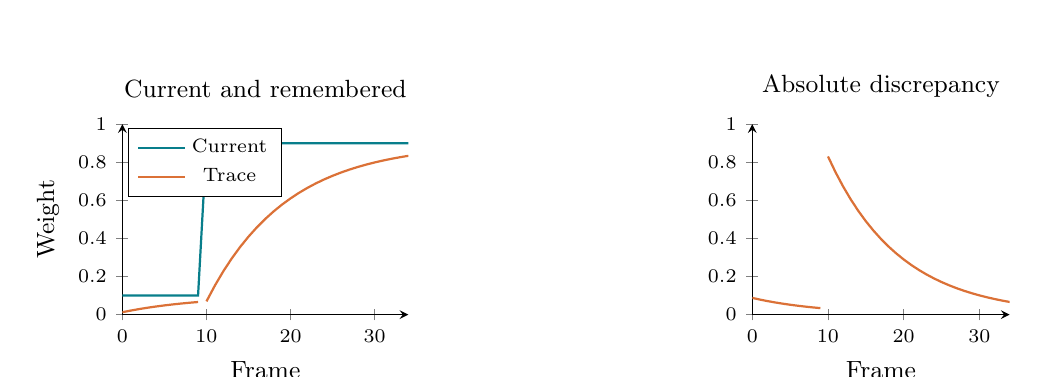
\begin{tikzpicture}
\begin{axis}[width=.43\linewidth,height=4.0cm,xmin=0,xmax=34,ymin=0,ymax=1,xlabel={Frame},ylabel={Weight},title={Current and remembered},legend style={font=\scriptsize,at={(.02,.98)},anchor=north west}]
\addplot[teal,thick]coordinates{(0,.1)(9,.1)(10,.9)(34,.9)};\addlegendentry{Current}
\addplot[orange,thick,domain=0:9,samples=10]{.1+(1/81-.1)*.9^x};
\addplot[orange,thick,domain=10:34,samples=25]{.9+(.1+(1/81-.1)*.9^10-.9)*.9^(x-10)};\addlegendentry{Trace}
\end{axis}
\begin{axis}[at={(8.0cm,0)},width=.40\linewidth,height=4.0cm,xmin=0,xmax=34,ymin=0,ymax=1,xlabel={Frame},title={Absolute discrepancy}]
\addplot[orange,thick,domain=0:9,samples=10]{abs((1/81-.1)*.9^x)};
\addplot[orange,thick,domain=10:34,samples=25]{abs((.1+(1/81-.1)*.9^10-.9)*.9^(x-10))};
\end{axis}\end{tikzpicture}\end{center}

{
\small\color{muted} Figure 5. Teaching simulation of one population coordinate, \(\eta\)=0.1 and r=1. The full model adds absolute differences over all 81 coordinates.\par}


After a stable motion changes, the current population moves toward different displacement candidates before the trace has caught up. That difference supplies a transient change signal. Over repeated observations the trace adapts, reducing the discrepancy. With a fixed effective update fraction 0.1, the influence of an old value decays by 0.9 per observation; its half-life is about 6.58 observations.


This trace and the next page's explicit time windows supply different descriptions. The trace has an exponentially fading history. The windows compare two finite, separated periods, preserving a defined earlier baseline for longer changes.


\clearpage

\section{Compare two periods locally}\label{sec12}

\textbf{The current population is pooled over a recent window and compared with an earlier reference window.}


\begin{equation}\mathcal W(t;w,g)=\{\max(0,t+1-g-w),\ldots,t-g\}\end{equation}

W names the included frame indices. w is the requested window width and g the count of most-recent frames excluded. A window is empty when its ending index is below zero. The recent window uses w=4, g=0; the reference uses w=8, g=8. Thus, once enough frames exist, recent covers t-3 through t and reference covers t-15 through t-8.


\begin{center}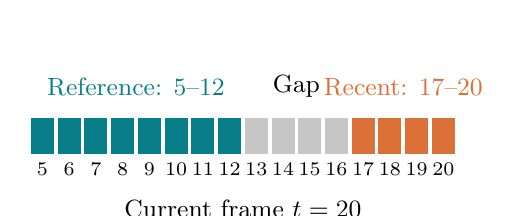
\begin{tikzpicture}[x=.028\linewidth,y=1cm]
\foreach \t in {5,...,20}{
\ifnum\t<13 \def\cc{teal}\else\ifnum\t<17 \def\cc{gray!45}\else\def\cc{orange}\fi\fi
\fill[\cc] (\t-.43,0) rectangle (\t+.43,.45);
\node[font=\scriptsize] at (\t,-.2){\t};}
\node[font=\small,text=teal] at (8.5,.85){Reference: 5--12};
\node[font=\small] at (14.5,.85){Gap};
\node[font=\small,text=orange] at (18.5,.85){Recent: 17--20};
\node[font=\small] at (12.5,-.7){Current frame $t=20$};
\end{tikzpicture}\end{center}

{
\small\color{muted} Figure 6. At t=20, reference frames 5-12 and recent frames 17-20 are separated by four unused frames, 13-16. The parameter gap=8 counts excluded recent frames, including the four-frame recent window.\par}


\begin{equation}\overline p_{t,\ell,i}^{(w,g)}=\frac{\sum_{s\in\mathcal W}r_{s,\ell,i}p_{s,\ell,i}}{\max(\sum_{s\in\mathcal W}r_{s,\ell,i},10^{-6})}\end{equation}

\begin{equation}a_{t,\ell,i}^{(w,g)}=\frac1w\sum_{s\in\mathcal W}r_{s,\ell,i}\end{equation}

Here s is a frame inside the window. The vector p-bar is a reliability-weighted average of its populations. The scalar a is the total reliability divided by the requested width. It records both signal strength and how much of the window is available. A full window of perfectly reliable observations gives a=1. A half-filled window with the same reliability gives a=0.5.


Name the earlier average R and the recent average O. These letters mean reference and observation. Their joint weight is \(\gamma\) = square root of (a\textsubscript{reference} times a\textsubscript{recent}). \(\gamma\) is zero when the reference has no observations. The first reference observation appears at t=8; it is frame zero. Full reference support appears at t=15. Therefore a seven-frame trial, t=0 through 6, has zero contribution from this explicit comparison branch.


Every quantity uses present or earlier observations. The windows run on every timestep with the same widths and gaps. They receive no cue times or change-event annotations. Cumulative sums implement these weighted boxcar averages efficiently.


\clearpage

\section{What the comparison stores}\label{sec13}

\textbf{Preserve the old pattern, the new pattern, and their differences at each location.}


\begin{equation}\gamma=\sqrt{a_Ra_O},\quad D_k=|O_k-R_k|,\quad d_1=\sum_kD_k\end{equation}

\begin{equation}d_{\cos}=1-\frac{\sum_k R_kO_k}{\max(\|R\|_2,10^{-8})\max(\|O\|_2,10^{-8})}\end{equation}

The site, time and lag indices are suppressed in these equations so the arithmetic is easier to read; all quantities still belong to one site and one lag. D is the 81-entry absolute difference. d\textsubscript{1} is its sum. The L2 norm ||R||\textsubscript{2} is square root of the sum of squared entries. The cosine compares the directions of the two vectors; subtracting it from one gives a shape difference.


\begin{center}\small\renewcommand{\arraystretch}{1.16}\setlength{\tabcolsep}{4pt}\begin{tabular}{p{0.349\linewidth}p{0.088\linewidth}p{0.463\linewidth}}\toprule

\textbf{Stored component across 3 lags} & \textbf{Count} & \textbf{Purpose} \\

\midrule

10\(\gamma\)R & 243 & Earlier local motion alternatives. \\

10\(\gamma\)O & 243 & Recent local motion alternatives. \\

10\(\gamma\)D & 243 & Which alternatives changed, coordinate by coordinate. \\

\(\gamma\)d1 & 3 & Overall absolute difference at each lag. \\

\(\gamma\)dcos & 3 & Population-shape difference at each lag. \\

Total per site & 735 & An explicit local comparison vector. \\

\bottomrule\end{tabular}\end{center}

The factor 10 is a fixed feature scale used for the population-valued components. It changes their magnitude before the learned readout; it is an engineering scale in this implementation. The scalar distances do not receive that factor. The same construction is repeated at all 100 image sites.


\subsection*{Why compare before pooling locations?}

Suppose a left site initially represents rightward motion and a right site initially represents leftward motion. They then swap. Averaging over locations first gives the same half-rightward, half-leftward population before and after. Comparing each location first exposes a change at both locations. Spatial attention can then select the comparison at the relevant site.


If both window populations are uniform, their difference is zero. If one is concentrated entirely on rightward motion and the other entirely on upward motion, d\textsubscript{1}=2 and d\textsubscript{cos}=1. These are teaching extremes; actual softmax outputs usually distribute weight over multiple alternatives.


\clearpage

\section{How motion reaches the answer}\label{sec14}

\textbf{The motion pathway feeds both fused visual tokens and explicit local comparisons, selected by the same attention weights.}


\begin{center}\small\renewcommand{\arraystretch}{1.16}\setlength{\tabcolsep}{4pt}\begin{tabular}{p{0.661\linewidth}p{0.239\linewidth}}\toprule

\textbf{Input to each visual token} & \textbf{Number of values} \\

\midrule

Learned appearance responses + raw RGB/\allowbreak{}RMS statistics & 32 + 4 \\

Motion populations scaled by 10r & 3 times 81 = 243 \\

Energy reliabilities r & 3 \\

Differences \(\delta\) from the adaptive trace & 3 \\

Expected horizontal/\allowbreak{}vertical velocities at 3 lags & 6 \\

Normalized pixel-prediction error \(\epsilon\) & 1 \\

Concatenated input /\allowbreak{} learned output & 292 /\allowbreak{} 64 \\

\bottomrule\end{tabular}\end{center}

\begin{equation}V_{t,i}=W_{\rm fusion}\phi_{t,i}+b_{\rm fusion}+e_i\end{equation}

The Greek letter \(\phi\) (phi) names the concatenated 292-entry feature list. W\textsubscript{fusion} is a learned 64 by 292 matrix; b is its learned 64-entry bias. e\textsubscript{i} is a learned position vector identifying site i. V is the resulting 64-entry visual token. Motion and appearance can influence the same token coordinates.


The recurrent attention module scores 100 site keys using one query derived from the previous global CLS memory. A softmax over sites gives weights \(\alpha\)\textsubscript{t,i}, which add to one. Each key depends on its current visual token and previous local spatial memory. Consequently, remembered information changes which current site is selected.


\begin{equation}b_t=\sum_{i=1}^{100}\alpha_{t,i}\,c_{t,i},\qquad m_t=0.8m_{t-1}+0.2b_t\end{equation}

c\textsubscript{t,i} is the 735-entry local comparison from section 13. b\textsubscript{t} is its attention-weighted spatial average. m\textsubscript{t} is the 735-entry comparison memory, initially zero. The same \(\alpha\) weights select learned visual values for the CLS update and modulate spatial memory writes. This is where the motion evidence participates in shared spatial selection.


At the final frame, the 64-entry CLS memory and the 735-entry comparison memory form a 799-entry vector. A learned linear layer and GELU turn it into 64 response features; the selected task head maps those features to answer logits. This separation allows the model to preserve detailed local motion comparisons alongside the compressed fused representation.


\clearpage

\section{A complete numerical walkthrough}\label{sec15}

\textbf{A synthetic texture moves right by exactly one pixel per frame; the fixed bank is executed unchanged.}


The input is a seeded 100 by 100 random grayscale texture, with values between 0.2 and 0.8. Each new frame translates the texture one pixel right. At frame 8, inspect site 44: row 4, column 4. This interior crop stays away from the image wrapping boundary. No trained checkpoint is used; refinement is initially zero and temperature is 0.04.


\begin{center}\small\renewcommand{\arraystretch}{1.16}\setlength{\tabcolsep}{4pt}\begin{tabular}{p{0.070\linewidth}p{0.208\linewidth}p{0.143\linewidth}p{0.129\linewidth}p{0.351\linewidth}}\toprule

\textbf{Lag} & \textbf{Largest-score shift} & \textbf{Score C} & \textbf{r} & \textbf{Mean velocity (x,y)} \\

\midrule

1 & (1, 0) & 0.98631 & 0.99540 & (1.0000, 0.0000) \\

2 & (2, 0) & 0.94733 & 0.99548 & (1.0000, 0.0000) \\

4 & (4, 0) & 0.81390 & 0.99562 & (1.0000, 0.0000) \\

\bottomrule\end{tabular}\end{center}

The peak displacement increases with elapsed time. Dividing by lag returns approximately the same one-pixel-per-frame velocity. The longer-lag score can be lower because the feature has moved farther under the fixed Hann window, and crop boundaries change the overlapping evidence.


\subsection*{Read the computation in sequence}

\textbf{1.} At each lag, retrieve the earlier crop and the current crop. Subtract their respective means and apply the same Hann window. \textbf{2.} Calculate 81 product sums and divide by the full-crop energy normalization. \textbf{3.} Convert the 81 scores into normalized weights with softmax. \textbf{4.} Weight the candidate shift coordinates by those values and divide by the lag. \textbf{5.} Average the three lag velocities to form the flow used for the next prediction.


\textbf{6.} Compare the current population with the old adaptive trace. \textbf{7.} Form the earlier and recent window populations where history exists. \textbf{8.} Supply motion features to fusion and supply local comparisons to shared attention. All these operations retain the location until the attention-weighted selection.


\subsection*{Checks executed for this document}

The actual CPU motion bank recovers maxima (1,0), (2,0), (4,0). Direct product sums match the FFT scores. A separate impulse-image check verifies the sign of backward sampling. A flat midpoint-gray movie gives zero score and zero reliability. The reference window is empty at t=7, has reliability mass divided by width equal to 1/\allowbreak{}8 at t=8, and reaches full support at t=15 when every frame is reliable.


{
\small\color{muted} All numerical outputs and source hashes are preserved in output/\allowbreak{}pdf/\allowbreak{}optic\_flow\_pathway\_verification.json. Synthetic demonstrations illustrate computation, rather than task accuracy.\par}


\clearpage

\section{The scientific ideas behind it}\label{sec16}

\textbf{Local motion evidence, distributed alternatives and normalization provide the theoretical starting points.}


\subsection*{Motion as orientation in space and time [5]}

Imagine a horizontal row of image pixels stacked over successive frames. A dot moving right traces a diagonal line in this space-time picture. The slope relates position change to elapsed time. Adelson and Bergen constructed motion-energy models with filters oriented in space-time: paired filter outputs are squared and summed, then opposite directions are compared. Their construction explains how direction selectivity can arise from image signals without assigning an identity to each dot.


Our connection is the underlying use of \textbf{spatial relationships across time}. The implemented bank measures alignment at explicit displacements and lags. Its central operation is the product-sum correlation derived above. The energy-model paper supplies a theoretical account of why spatiotemporal structure supports motion sensing.


\subsection*{A population can retain ambiguity [6]}

Simoncelli and Heeger modeled responses in visual areas V1 and MT through weighted inputs, rectification and normalization. Their model represents local velocity using a distribution of neuronal responses. A population permits multiple directions and speeds to be expressed together; the pattern across units carries information that a single winning unit would discard.


In our implementation, the 81 coordinates have explicitly assigned displacements. Keeping their joint pattern is useful when the image supports multiple matches. The expected velocity is one summary of that pattern. The larger population remains available for detecting changes even when opposing alternatives cancel in the mean.


\subsection*{Normalization separates two questions}

The crop-energy denominator asks how well the prepared structures align relative to their scale. The reliability factor separately carries their signal strength. This is an engineering decomposition motivated by a common computational need: preserve which alternative fits while controlling the effect of input magnitude. The code states exactly how the two quantities are constructed.


\subsection*{Learning uses both prediction and the task}

The pixel objective rewards a flow that predicts continuing image structure. The response objective rewards representations useful for the behavioral judgment. Together they can shape refinement and selection. The finite crop, candidate grid, chosen lags and temporal windows specify the problems that learning is asked to solve within this architecture.


\clearpage

\section{Fixed rules and learned quantities}\label{sec17}

\textbf{The method combines an explicit correspondence calculation with trainable interpretation.}


\begin{center}\small\renewcommand{\arraystretch}{1.16}\setlength{\tabcolsep}{4pt}\begin{tabular}{p{0.395\linewidth}p{0.239\linewidth}p{0.266\linewidth}}\toprule

\textbf{Component} & \textbf{Fixed or learned?} & \textbf{Role} \\

\midrule

24-pixel crop; stride 10; Hann window & Fixed & Defines local image support. \\

Lags 1, 2, 4; shifts -4 to +4 & Fixed & Defines the measured temporal/\allowbreak{}spatial alternatives. \\

FFT correlation and energy normalization & Fixed arithmetic & Produces image-derived match scores. \\

1 to 4 to 1 convolutional refinement & Learned: 77 parameters & Adjusts local structure in displacement-score space. \\

Three temperatures & Learned, bounded & Controls sharpness separately at each lag. \\

Adaptive-trace update fraction & Learned scalar & Controls rate of adaptation. \\

Window widths/\allowbreak{}gaps and comparison decay 0.8 & Fixed & Specifies explicit temporal comparisons. \\

Fusion, recurrent attention and response layers & Learned & Uses motion and appearance to solve the task. \\

\bottomrule\end{tabular}\end{center}

The first refinement convolution has 4 times 1 times 3 times 3 weights plus four biases, giving 40 parameters. The second has 1 times 4 times 3 times 3 weights plus one bias, giving 37. Together with three temperatures and one trace-rate parameter, these add 81 learned parameters around the fixed motion computations. Fusion and recurrent processing contain additional learned parameters.


\subsection*{Why these pieces fit together}

Raw differences between images mix motion with changes in appearance. Correlation instead evaluates candidate correspondences. The population preserves alternatives; the mean provides a compact displacement. Prediction tests temporal continuation; traces and windows detect changes in evidence. Shared attention identifies which local evidence should influence memory. The task head translates the selected memory into its response vocabulary.


This arrangement builds correspondence and temporal comparison into the representation. Those choices explain the pathway's usefulness and define concrete things to test: shift range versus stimulus speed, crop size versus object size, lag versus dot lifespan, and window support versus trial duration. Each test changes a specific part of the computational chain.


\clearpage

\section{Symbol and units reference}\label{sec18}

\textbf{The same symbols keep the same roles across this document.}


\begin{center}\small\renewcommand{\arraystretch}{1.16}\setlength{\tabcolsep}{4pt}\begin{tabular}{p{0.187\linewidth}p{0.428\linewidth}p{0.285\linewidth}}\toprule

\textbf{Symbol} & \textbf{Meaning} & \textbf{Shape /\allowbreak{} units} \\

\midrule

X; I & RGB input; channel-mean grayscale & 3 x 100 x 100; 100 x 100 per frame \\

t; \(\ell\); i & Frame index; lag; spatial site & Integer; frame steps; 0-99 \\

x,y; a,b & Image coordinates; crop coordinates & Pixels; integers 0-23 \\

Q; P & Extracted centered crop; prepared crop & 24 x 24 each \\

w; N; C & Hann weight; raw correlation; normalized score & Scalar at each coordinate or shift \\

E; z; r & Prepared crop energy; joint energy; reliability & Scalar; scalar; fraction in [0,1) \\

p; \(\tau\) & Displacement population; temperature & 81 weights per site/\allowbreak{}lag; positive scalar \\

d; v; f & Displacement; lag velocity; mean-lag flow & 2D: pixels; pixels/\allowbreak{}frame; pixels/\allowbreak{}frame \\

I-hat; \(\epsilon\); \(\omega\) & Predicted image; normalized error; loss weight & Image; scalar/\allowbreak{}site; scalar/\allowbreak{}site \\

h; \(\eta\); \(\delta\) & Population trace; trace update rate; L1 distance & 81 values; fraction; scalar/\allowbreak{}site/\allowbreak{}lag \\

R; O; \(\gamma\) & Reference; recent population; joint support & 81 values each; scalar/\allowbreak{}site/\allowbreak{}lag \\

c; \(\alpha\); m & Local comparison; attention; comparison memory & 735/\allowbreak{}site; fraction/\allowbreak{}site; 735 global \\

\(\phi\); V & Concatenated features; fused token & 292/\allowbreak{}site; 64/\allowbreak{}site \\

\bottomrule\end{tabular}\end{center}

E denotes a sum of prepared squared values on section 5, whereas e on section 10 denotes an average squared deviation from fixed gray over a smaller block. These two energy measurements use different spatial supports and centering rules. The position vector e\textsubscript{i} on section 14 is explicitly labeled there; its 64-entry shape distinguishes it from the scalar image energy e\textsubscript{t,i}.


{
\small\color{muted} Reading operators: |x| is absolute value; ||v||2 is square root of the sum of squared entries; exp is the exponential; max(a,b) chooses the larger value; a subscript selects an index; a superscript can label a component or window. The arithmetic meaning is specified immediately below each equation.\par}


\clearpage

\section{Where the spatial numbers come from}\label{sec19}

\textbf{Separate chosen settings, derived counts, and quantities that training adjusts.}


A fixed setting specifies the calculation we elected to perform. A derived number follows arithmetically from those settings. A learned value is adjusted by optimization, although its initialization and bounds can still be chosen. Stating these categories makes the method reproducible and makes each design decision available for testing.


\begin{center}\small\renewcommand{\arraystretch}{1.16}\setlength{\tabcolsep}{4pt}\begin{tabular}{p{0.202\linewidth}p{0.220\linewidth}p{0.478\linewidth}}\toprule

\textbf{Number} & \textbf{Origin} & \textbf{Reason and consequence} \\

\midrule

100 by 100 input & Chosen input format & The present backbone accepts this resolution. It establishes the coordinate scale for every pixel displacement. \\

Stride 10; 10 by 10 sites; 100 sites & 10 chosen; grid dimensions derived & Stride sets spacing. With the implemented padding and crop size, floor((100+14-24)/\allowbreak{}10)+1 = 10 sites per axis; 10 squared = 100. \\

24 by 24 crops & Chosen spatial support & Larger crops supply more correspondence evidence; smaller crops provide more local measurements. \\

Padding 7 per side & Alignment choice consistent with crop and stride & (24-10)/\allowbreak{}2=7 aligns crop centers with the 10-pixel blocks. Neighboring crops share 24-10=14 columns. \\

Radius 4; nine offsets; 81 pairs & 4 chosen; 9 and 81 derived & Search extent is limited to four pixels per component. Nine integer offsets include both endpoints and zero; nine squared = 81. \\

FFT side length 32 & Chosen computational size & Power-of-two size above 24. Its eight zero-padded positions per axis suffice for exact finite-crop correlation at retained shifts up to four pixels. \\

Hann denominator 23 & Derived from 24 samples & Indices 0 through 23 place both endpoints at zero in the nonperiodic Hann formula. \\

Integer shift spacing 1 pixel & Chosen candidate discretization & Softmax expectations can be fractional even though individual candidates lie on this integer grid. \\

\bottomrule\end{tabular}\end{center}

The earlier CorrespondencePredictiveMemory implementation used 50-pixel crops, a 25-pixel stride, FFT side 64 and radius 10, giving 441 displacement pairs. The current values belong to a different local representation. That historical difference documents a design change; the inspected notes do not establish that radius 4 is an optimum.


\clearpage

\section{Where the temporal and scale numbers come from}\label{sec20}

\textbf{Their computational effects are explicit; their particular values are design settings.}


\begin{center}\small\renewcommand{\arraystretch}{1.16}\setlength{\tabcolsep}{4pt}\begin{tabular}{p{0.206\linewidth}p{0.224\linewidth}p{0.470\linewidth}}\toprule

\textbf{Setting} & \textbf{Origin} & \textbf{What the setting controls} \\

\midrule

Lags 1, 2, 4 & Chosen frame intervals & Samples different temporal separations. Maximum represented component speed is R divided by lag: 4, 2 and 1 pixels per frame at R=4. \\

Recent width 4; reference width 8; gap parameter 8 & Chosen temporal windows & Compares recent evidence with an older baseline. The four intervening frames follow from 8 excluded recent frames minus the four-frame recent window. \\

Trace rate initially 0.1 & Chosen initialization; learned thereafter & Initial adaptation is 10\% per reliable observation. The actual update also multiplies by reliability. \\

Comparison memory decay 0.8; update 0.2 & 0.8 chosen; 0.2 = 1-0.8 & Retains 80\% of the previous comparison memory and adds 20\% of the current selected vector. \\

Temperature initially 0.04; bounds 0.015-0.2 & Initialization and bounds chosen; temperature learned & Sets the sensitivity of softmax weights to score differences. \\

Refinement multiplier 0.1; population multiplier 10 & Chosen feature scales & Scales the learned correction and the population features. These coefficients specify the relative magnitudes presented to subsequent computation. \\

Energy offsets 0.01 and 0.0001 & Chosen reliability scales & A ratio z/\allowbreak{}(z+c) equals one half when z=c. The constants set that half-weight energy scale for two different energy definitions. \\

Floors 1e-8, 1e-6, 1e-4 & Chosen numerical safeguards & Prevent tiny denominators in correlation/\allowbreak{}cosine, temporal averaging and pixel error. Each floor belongs to its explicitly stated equation. \\

Pixel loss multiplier 0.05 & Chosen objective weight & Sets the contribution of image prediction relative to the behavioral loss. \\

\bottomrule\end{tabular}\end{center}

These statements explain the role of each choice. Evidence that one value is preferable would require a controlled comparison, keeping data, compute and evaluation consistent. The present implementation supplies the values and their effects; it does not contain an optimization study of every constant.


\clearpage

\section{References and code provenance}\label{sec21}

\textbf{Primary sources explain the ideas; the inspected source code defines the implemented equations.}


\textbf{[1] Dosovitskiy, A. et al. (2015). FlowNet: Learning Optical Flow with Convolutional Networks. ICCV.}


{
\small\color{muted} \href{https://arxiv.org/abs/1504.06852}{https:/\allowbreak{}/\allowbreak{}arxiv.org/\allowbreak{}abs/\allowbreak{}1504.06852}\par Connection: correlation volumes expose matching evidence to learned processing.\par}


\textbf{[2] PyTorch. torch.fft.irfft2 documentation.}


{
\small\color{muted} \href{https://docs.pytorch.org/docs/2.14/generated/torch.fft.irfft2.html}{https:/\allowbreak{}/\allowbreak{}docs.pytorch.org/\allowbreak{}docs/\allowbreak{}2.14/\allowbreak{}generated/\allowbreak{}torch.fft.irfft2.html}\par API reference for the real inverse transform. Local numerical checks verify the running implementation.\par}


\textbf{[3] PyTorch. torch.nn.functional.grid\_sample documentation.}


{
\small\color{muted} \href{https://docs.pytorch.org/docs/2.14/generated/torch.nn.functional.grid_sample.html}{https:/\allowbreak{}/\allowbreak{}docs.pytorch.org/\allowbreak{}docs/\allowbreak{}2.14/\allowbreak{}generated/\allowbreak{}torch.nn.functional.grid\_sample.html}\par API reference for source coordinates, bilinear sampling, border handling and align\_corners.\par}


\textbf{[4] Jaderberg, M., Simonyan, K., Zisserman, A. and Kavukcuoglu, K. (2015). Spatial Transformer Networks. NeurIPS.}


{
\small\color{muted} \href{https://arxiv.org/abs/1506.02025}{https:/\allowbreak{}/\allowbreak{}arxiv.org/\allowbreak{}abs/\allowbreak{}1506.02025}\par Connection: differentiable sampling allows image errors to influence spatial transformations.\par}


\textbf{[5] Adelson, E. H. and Bergen, J. R. (1985). Spatiotemporal energy models for the perception of motion. JOSA A 2(2), 284-299.}


{
\small\color{muted} \href{https://doi.org/10.1364/JOSAA.2.000284}{https:/\allowbreak{}/\allowbreak{}doi.org/\allowbreak{}10.1364/\allowbreak{}JOSAA.2.000284}\par Connection: direction-sensitive computations from image structure across space and time.\par}


\textbf{[6] Simoncelli, E. P. and Heeger, D. J. (1998). A model of neuronal responses in visual area MT. Vision Research 38(5), 743-761.}


{
\small\color{muted} \href{https://www.cns.nyu.edu/pub/eero/simoncelli96.pdf}{https:/\allowbreak{}/\allowbreak{}www.cns.nyu.edu/\allowbreak{}pub/\allowbreak{}eero/\allowbreak{}simoncelli96.pdf}\par Connection: distributed motion representation and normalization in a model of V1/\allowbreak{}MT.\par}


\subsection*{Implementation record}

{
\small\color{muted} Verified October 12, 2026 against continuation07/\allowbreak{}config.json source\_sha256. The actual suite inherits the stabilized backbone through StabilizedAttentionSuite and StabilizedAttentionVDA. Local training uses PyTorch 1.13.1+cu117; the cited API pages are current documentation. The sign, normalization and startup claims were also checked directly on CPU with the local library.\par}


{
\small\color{muted} Source entry points: StabilizedAttentionKrauzlis/\allowbreak{}model.py: LocalMotionBank (lines 14-36), warp (39-45), causal\_average (48-60), population/\allowbreak{}comparison construction (96-114), prediction/\allowbreak{}trace/\allowbreak{}fusion (117-141), attention routing (155-171). MemoryGuidedSearch/\allowbreak{}train.py: update(), task loss plus 0.05 prediction loss. Full paths and SHA256 values are recorded in the companion verification JSON.\par}

\end{document}
